\documentclass[a4paper, 11pt]{article}
\usepackage{graphicx}
\title{CCTBX for Diffraction Calculations 1}
\author{Graeme Winter, Diamond Light Source}

\begin{document}

\maketitle

\section{Introduction}

The CCTBX toolbox (http://cctbx.sourceforge.net) is a hybrid C++ / Python library for the development of crystallographic applications with an emphasis on rapid prototyping. The original emphasis of the library was for calculations relating to crystallographic refinement, which is evident from the examples shown on the main web page. Otherwise however the documentation is sparse. The purpose of this introduction is to show the application of the library to several commonly needed diffraction calculations, by developing a tool to compute a map from an image of the squared distance from each pixel to the nearest reciprocal space node, given a properly defined imgCIF file and an orientation matrix.

\section{Getting Started}

The only pre-requisites of following this document are installing cctbx (from the web page above) and obtaining the example data file (included with this document.) The file is relatively tiny (it was recorded on a Pilatus 300K used for small molecule crystallography) and self-contained so there are no further requirements. 

\section{Reading the File}

The input file is in full imgCIF / CBF format, which means that the full experimental geometry is embedded within the file. This has the advantages that (i) no external dependencies are there and (ii) we know what the description of the geometry means. This in turn makes life very straightforward. 

Accessing the file simply requires:

{\small
\begin{verbatim}
import pycbf

...

    cbf_handle = pycbf.cbf_handle_struct()
    cbf_handle.read_file(cbf_image, pycbf.MSG_DIGEST)
\end{verbatim}
}

\noindent
Getting hold of additional information about the detector and goniometer requires a little more effort:

{\small
\begin{verbatim}
def find_beam_direction(cbf_handle):
    '''Find the beam direction (why is this not simpler in pycbf?)'''

    cbf_handle.find_category('axis')
    cbf_handle.find_column('equipment')
    cbf_handle.find_row('source')

    beam_direction = []

    for j in range(3):
        cbf_handle.find_column('vector[%d]' % (j + 1))
        beam_direction.append(cbf_handle.get_doublevalue())

    B = - matrix.col(beam_direction).normalize()

    return B
\end{verbatim}
}

\noindent
It is important to note that in imgCIF, the direction of the recorded beam direction is from the sample, towards the source. This is the exact opposite of $S_0$ in e.g. Giacovazzo. This however shows the first usage of the cctbx \verb|matrix.col| class - instantiated from a list then normalized to give a unit vector.

The next step is to find out information about the detector: the position and orientation, the dimensions and the size of the pixels:

{\small
\begin{verbatim}
    detector = cbf_handle.construct_detector(0)

    # this returns slow fast slow fast pixels pixels mm mm
    detector_normal = tuple(detector.get_detector_normal())
    distance = detector.get_detector_distance()
    pixel = (detector.get_inferred_pixel_size(1),
             detector.get_inferred_pixel_size(2))

    # this method returns slow then fast dimensions i.e. (y, x)

    size = tuple(reversed(cbf_handle.get_image_size(0)))

    wavelength = cbf_handle.get_wavelength()

    O = matrix.col(detector.get_pixel_coordinates(0, 0))
    fast = matrix.col(detector.get_pixel_coordinates(0, 1))
    slow = matrix.col(detector.get_pixel_coordinates(1, 0))

    X = fast - O
    Y = slow - O

    X = X.normalize()
    Y = Y.normalize()
    N = X.cross(Y)

    S0 = (1.0 / wavelength) * B
\end{verbatim}
}

\noindent
In this context this is sufficient information, however care should be taken to ensure that the resulting properties are interpreted \emph{in the correct order} e.g. fast / slow or vice versa.

For this calculation the only information we need from the goniometer is the effect that all of the settings will have in the middle of the frame. This is most easily expressed as a matrix calculated from the goniometer handle thus:

{\small
\begin{verbatim}
    gonio = cbf_handle.construct_goniometer()
    x = gonio.rotate_vector(0.5, 1, 0, 0)
    y = gonio.rotate_vector(0.5, 0, 1, 0)
    z = gonio.rotate_vector(0.5, 0, 0, 1)

    R = matrix.sqr(x + y + z).transpose()
\end{verbatim}
}

\noindent
This rotates the vectors $i$, $j$, $k$ to determine the effects of the rotation settings then constructs a matrix from these, the transpose of which (i.e. inverse) is needed.

\section{Real Calculations}

At this stage we now have a full mathematical description of the experimental geometry, so are well set to get stuck in to the calculation of the distance map. Starting from: $x = R U B h$ we want to obtain $h$ from pixel positions. Thus, $(R U B)^{-1}$ is needed:

{\small
\begin{verbatim}
    # This was the known UB matrix, derived from XDS processing.

    UB = matrix.sqr([0.0144873, -0.0128813, -0.0002988,
                    -0.0128113, -0.0143530, -0.0024004,
                     0.0013736,  0.0019910, -0.0192366])
    RUBI = (R * UB).inverse()
\end{verbatim}
}

\noindent
where we previously obtained the $U B$ matrix from processing the data. From here we're nearly done. As we want to compute an ``image'' of the distances, simply keeping the distances in a list in the right order and the size of the array is adequate. The calculation of the reciprocal space position itself and squared distance is straightforward:

{\small
\begin{verbatim}
            p = matrix.col(detector.get_pixel_coordinates(j, i)).normalize()
            q = (1.0 / wavelength) * p - S0
            _hkl = (RUBI * q).elems
            hkl = map(nint, _hkl)

            d2 = sum([(_hkl[k] - hkl[k]) * (_hkl[k] - hkl[k])
                      for k in range(3)])
\end{verbatim}
}

\section{Plotting}

Though matplotlib is formally not a part of cctbx, it is included in some bundles. This can be used as follows:

{\small
\begin{verbatim}
def plot_image(size1, size2, image_values):
    '''Plot an image size size1 x size2 of values.'''

    from matplotlib import pyplot as plt
    import numpy

    assert(len(image_values) == size1 * size2)

    image = numpy.reshape(numpy.array(image_values, dtype = float),
                          (size1, size2))

    plt.imshow(image)
    plt.savefig('cctbx_introduction_1.png')

    return
\end{verbatim}
}

\noindent
Which when added to the code in \verb|cctbx_introductin_1.py| gives:

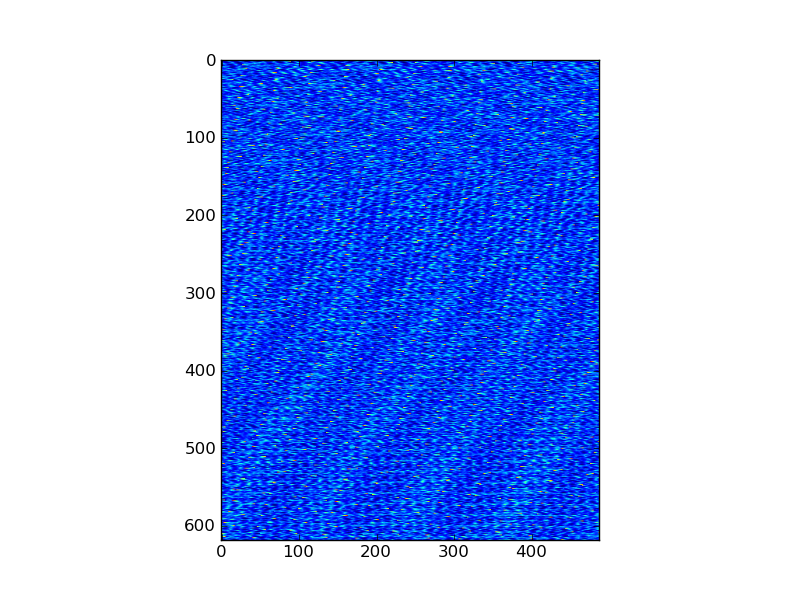
\includegraphics[scale = 0.5]{cctbx_introduction_1.png}

\end{document}